\documentclass{article}
\usepackage[T1]{fontenc}
\usepackage{lmodern}
\usepackage{graphicx}
\usepackage{amsmath,amssymb}
\usepackage[a4paper,margin=2cm]{geometry}
\usepackage[absolute,overlay]{textpos}
\setlength{\TPHorizModule}{1mm}
\setlength{\TPVertModule}{1mm}
\usepackage[indonesian]{babel}
\usepackage{hyperref}
\setlength{\emergencystretch}{2em}
% unit: Halaman 75

\begin{document}

% === Halaman 75 (llm) ===

\vspace{100.98mm}

\begin{tabular}{|l|c|c|c|}
\hline
Register length & Feedback bit & Feedforward bit & AND inputs \\ \hline
 A & 93 & 69 & 66 & 91, 92 \\ \hline
 B & 84 & 78 & 69 & 82, 83 \\ \hline
 C & 111 & 87 & 66 & 109, 110 \\ \hline
\end{tabular}

% deskripsi: Diagram sirkuit aliran data untuk generator key stream yang terdiri dari tiga register geser (A, B, C) dengan operasi XOR dan gerbang AND sebagai feedback dan feedforward.
% bbox normalisasi: [0.1100, 0.3000, 0.7300, 0.6400]
\begin{textblock*}{130.20mm}(23.10mm,89.10mm)
\noindent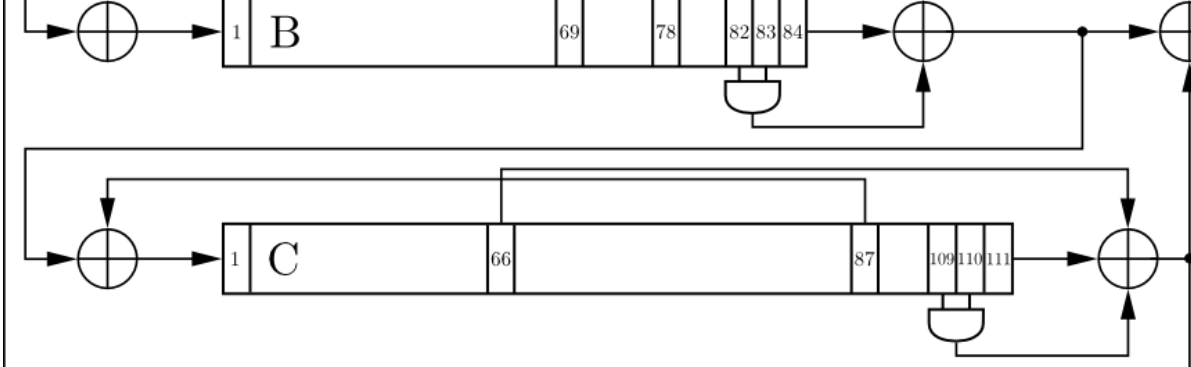
\includegraphics[width=130.20mm,height=100.98mm]{../../images/llm/page_075_img_01.png}%
\end{textblock*}

\end{document}
